\subsubsection{Problem 2}
In this problem, the purpose was to track a multivariable reference
\begin{equation}\label{eq:P3_p2_reference}
    \mathbf{r}=
        \begin{bmatrix}
            \tilde{p_c}\\
            \dot{\tilde{e_c}}
        \end{bmatrix}.
\end{equation}
Firstly, the controllability of the system is examined. Due to \cref{eq:P3_state_vector_and_input} having three states, the controllability matrix is given by
\begin{equation}\label{eq:P3_p2_controllability_matrix}
    \mathcal{C}=
        \begin{bmatrix}
            \mathbf{B}&\mathbf{AB}&\mathbf{A^2B}
        \end{bmatrix}
        =
        \begin{bmatrix}
            0   &   0   &  K_1 &0&0&0 \\
            K_1 &   0   &  0   &0&0&0 \\
            0   &   K_2 &  0   &0&0&0
        \end{bmatrix}.
\end{equation}
With the values $K_1=0.9046$ and $K_2=0.1555$ inserted, this becomes 
\begin{equation}
    \mathcal{C}=
        \begin{bmatrix}
            0      &   0      &  0.9046 &0&0&0 \\
            0.9046 &   0      &  0      &0&0&0 \\
            0      &   0.1555 &  0      &0&0&0
        \end{bmatrix}.
\end{equation}
\begin{figure}[!!ht!!!!!!!!tb!!]
	\centering
		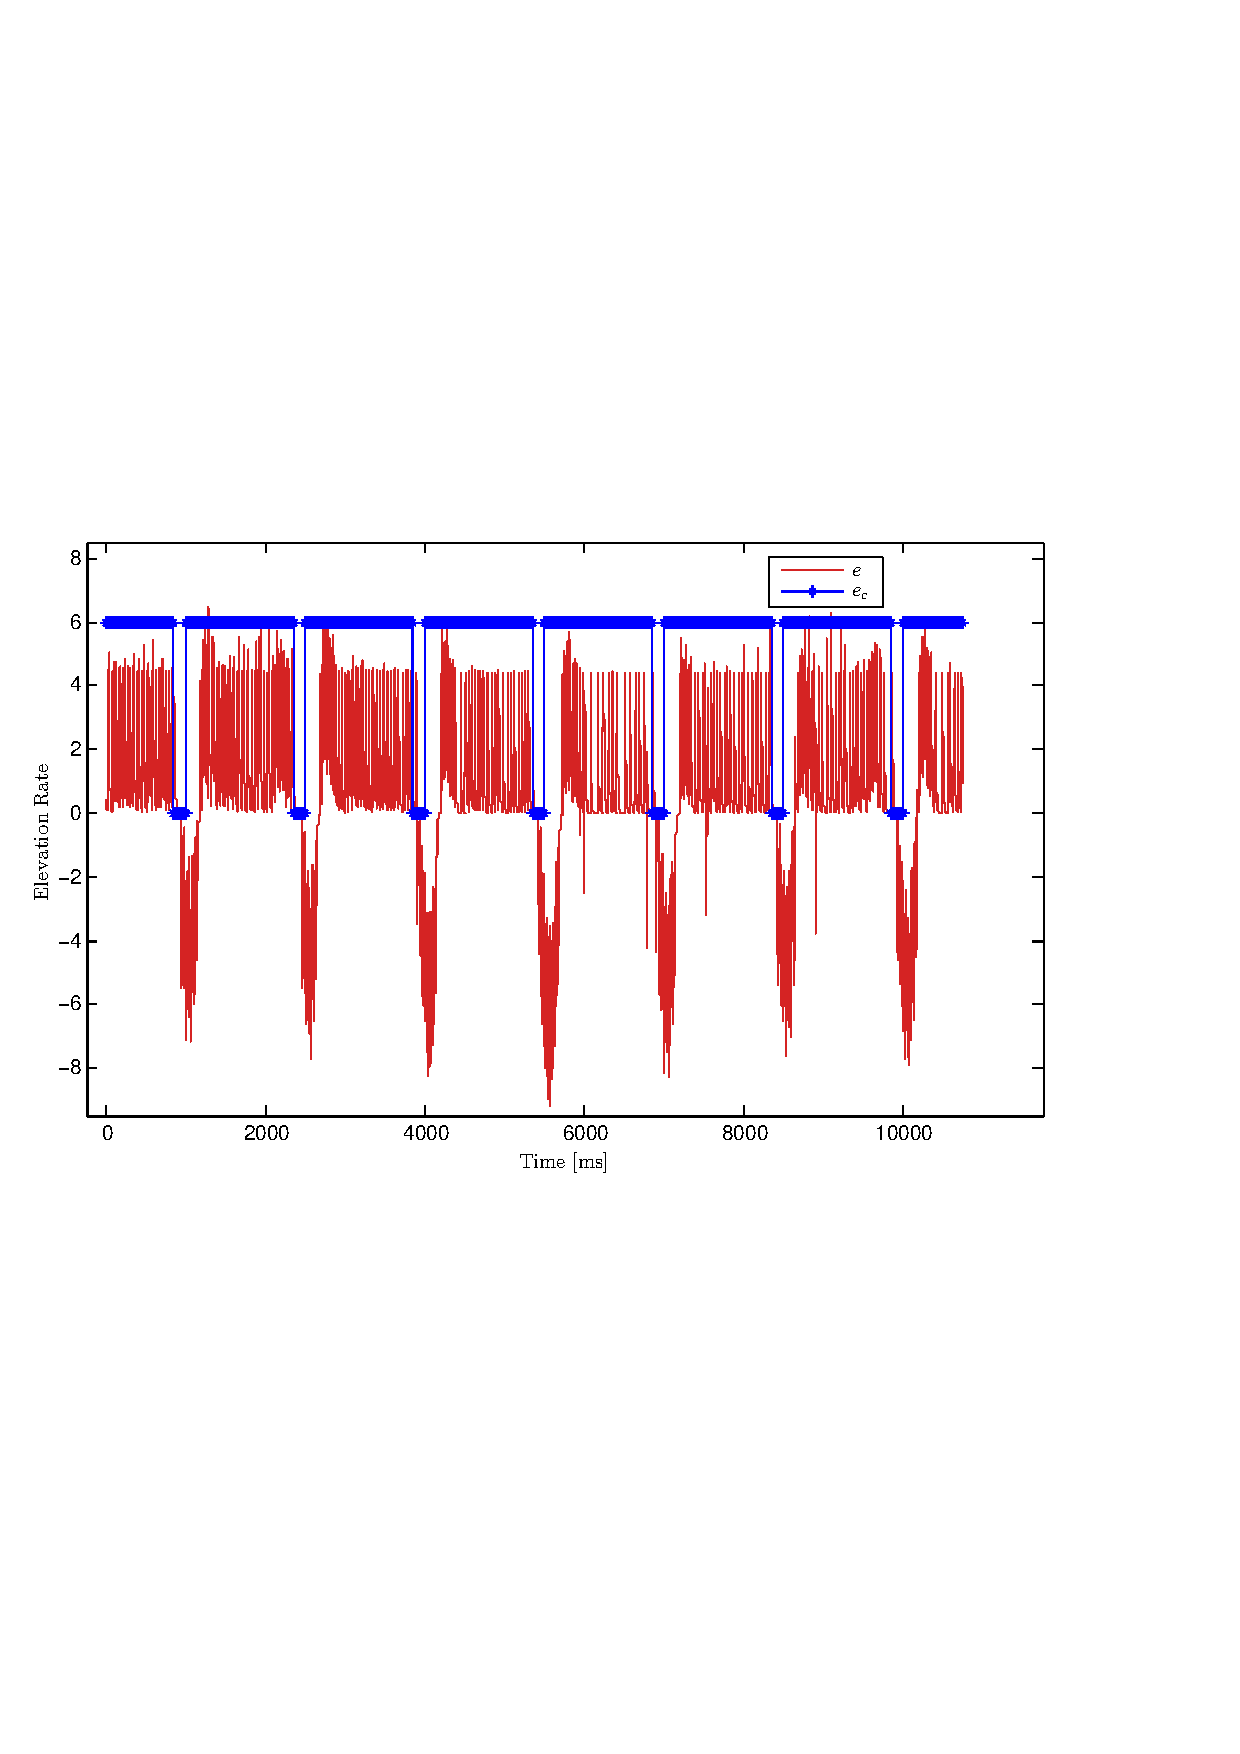
\includegraphics[width=1\textwidth,trim={4cm 9cm 4cm 9cm},clip]{figures/P3p2_e_dot.pdf}
	\caption{Travel response with P control}
\label{fig:P3p2_e_dot}
\end{figure}
\clearpage
\begin{figure}[!!ht!!!!!!!!tb!!]
	\centering
		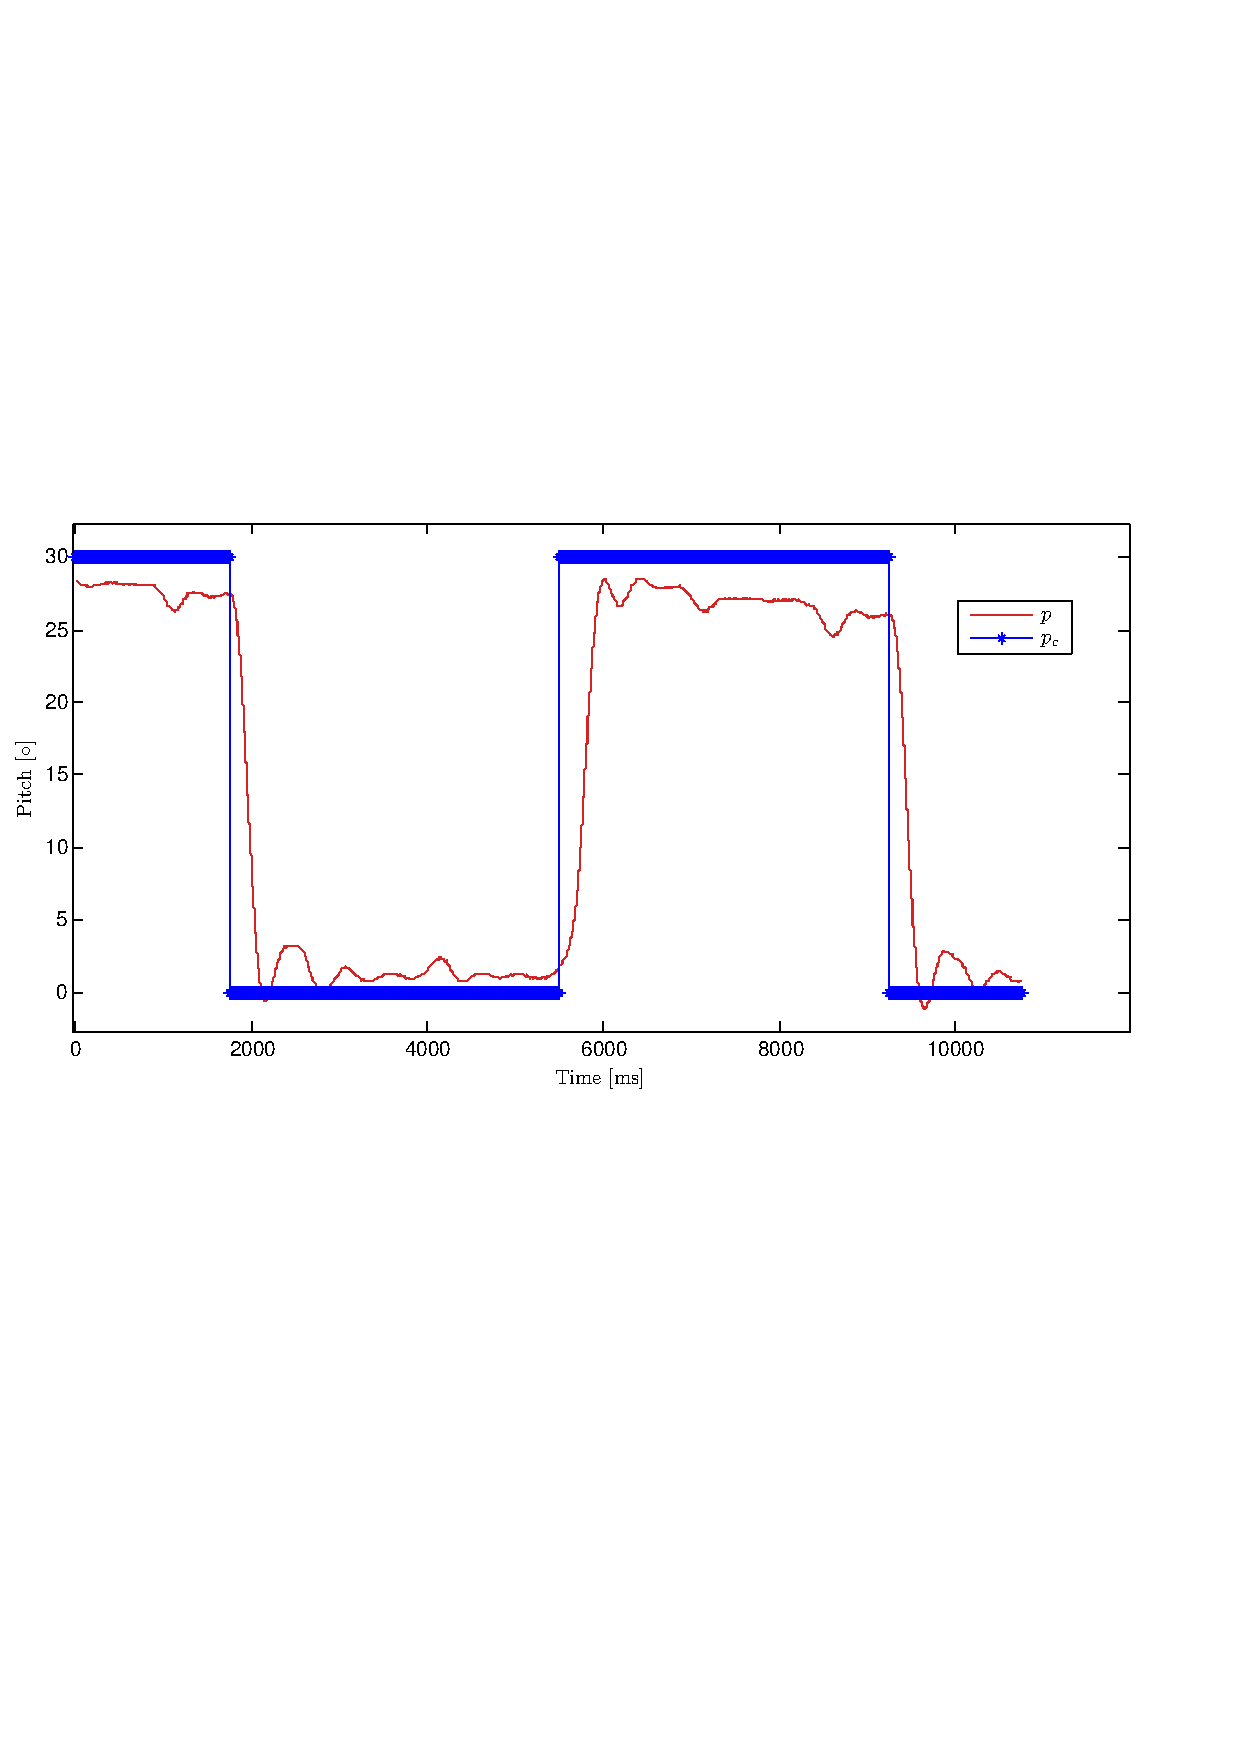
\includegraphics[width=1\textwidth,trim={4cm 9cm 4cm 9cm},clip]{figures/P3p2_p.pdf}
	\caption{Travel response with P control}
\label{fig:P3p2_p}
\end{figure}
\clearpage
